\section{Generation, Rendering, and Quality Control}
\label{sec:quality}

\subsection{Sampling and prompt realization}

\trace samples tasks uniformly by default and samples semantic query branches
within each task. Task generators construct unique answers rather than
relaxing constraints after failure. Prompt realization composes versioned
scene, task, optional query, and output-mode templates, with the selected
realization retained for replay. Visible labels, styles, layouts, and
distractors vary independently where the scene permits.

\subsection{Factorized instance variation}

\trace separates controls by what they are allowed to change. Semantic
instance controls include board and grid dimensions; object, mark, category,
series, panel, and node counts; numerical values and thresholds; path or
action-sequence lengths; and candidate-set cardinality. These controls may
change the latent state, answer, and empirical difficulty of an instance, but
must preserve the scene grammar, reasoning program, answer type, and verifier
semantics of its task.

The remaining controls realize a fixed semantic instance. They include
placement and spacing, panel arrangement, answer-preserving camera and
framing choices, palette, typography, materials, contextual text, and bounded
raster effects. This classification is task-dependent: placement, layout, or
camera is semantic whenever the task queries it, and is render-only only when
the same latent relations and answer are preserved. Table~\ref{tab:variation-layers}
summarizes these boundaries.

\begin{table}[h]
  \centering
  \small
  \setlength{\tabcolsep}{4pt}
  \renewcommand{\arraystretch}{1.12}
  \caption{Variation layers and the invariants they must preserve.}
  \label{tab:variation-layers}
  \begin{tabular}{@{}p{0.21\linewidth}p{0.44\linewidth}p{0.25\linewidth}@{}}
    \toprule
    Layer & Representative controls & Required invariant \\
    \midrule
    Semantic instance
      & Dimensions, cardinalities, values, operation length, candidate set
      & Scene and task contract \\
    Structural realization
      & Placement, spacing, panel arrangement, framing, answer-preserving camera
      & Latent relations and answer \\
    Surface and context
      & Palette, typography, skins, materials, labels, non-answer text
      & Latent state and answer \\
    Post-render
      & Blur, resampling, compression, tone, noise, texture
      & Canvas geometry and answer \\
    \bottomrule
  \end{tabular}
\end{table}

\subsection{Layered visual realization}

Once semantic execution fixes the objects, values, relations, and answer, the
renderer resolves only scene-compatible structural and surface controls.
Figure~\ref{fig:rendering-variation} shows this separation directly: one
node-link graph instance is realized under different palettes, typography,
layout, non-answer context, and raster noise while retaining the same prompt,
topology, query, and typed answer. Admissible controls remain scene-specific; for
example, a dashboard can vary report framing, whereas a board game can vary
board skins and piece appearance while retaining its game state.

Information-rich scenes can also sample controlled non-answer context from
curated text pools, including titles, captions, source notes, sidebars, metric
snippets, and paragraph boxes. Compatible scenes select among clean, minimal,
and report-style compositions; context is sampled independently of the answer
and query and is excluded from the reasoning contract. Context elements are
placed only where fit, collision, and contrast checks pass, and their role,
text, source, and bounding box are retained in the execution trace. This makes
textual clutter auditable, but does not by itself establish robustness to such
clutter.

Answer-bearing geometry is used for verifier projections and for visibility,
contrast, collision, and fit checks. Optional context and bounded raster
effects preserve the task contract, and each stochastic choice is
drawn from an independent seeded stream and recorded for replay.
Appendix~\ref{app:generation}
provides the corresponding control-flow diagram and domain-level variation
summary.

\begin{figure*}[t]
  \centering
  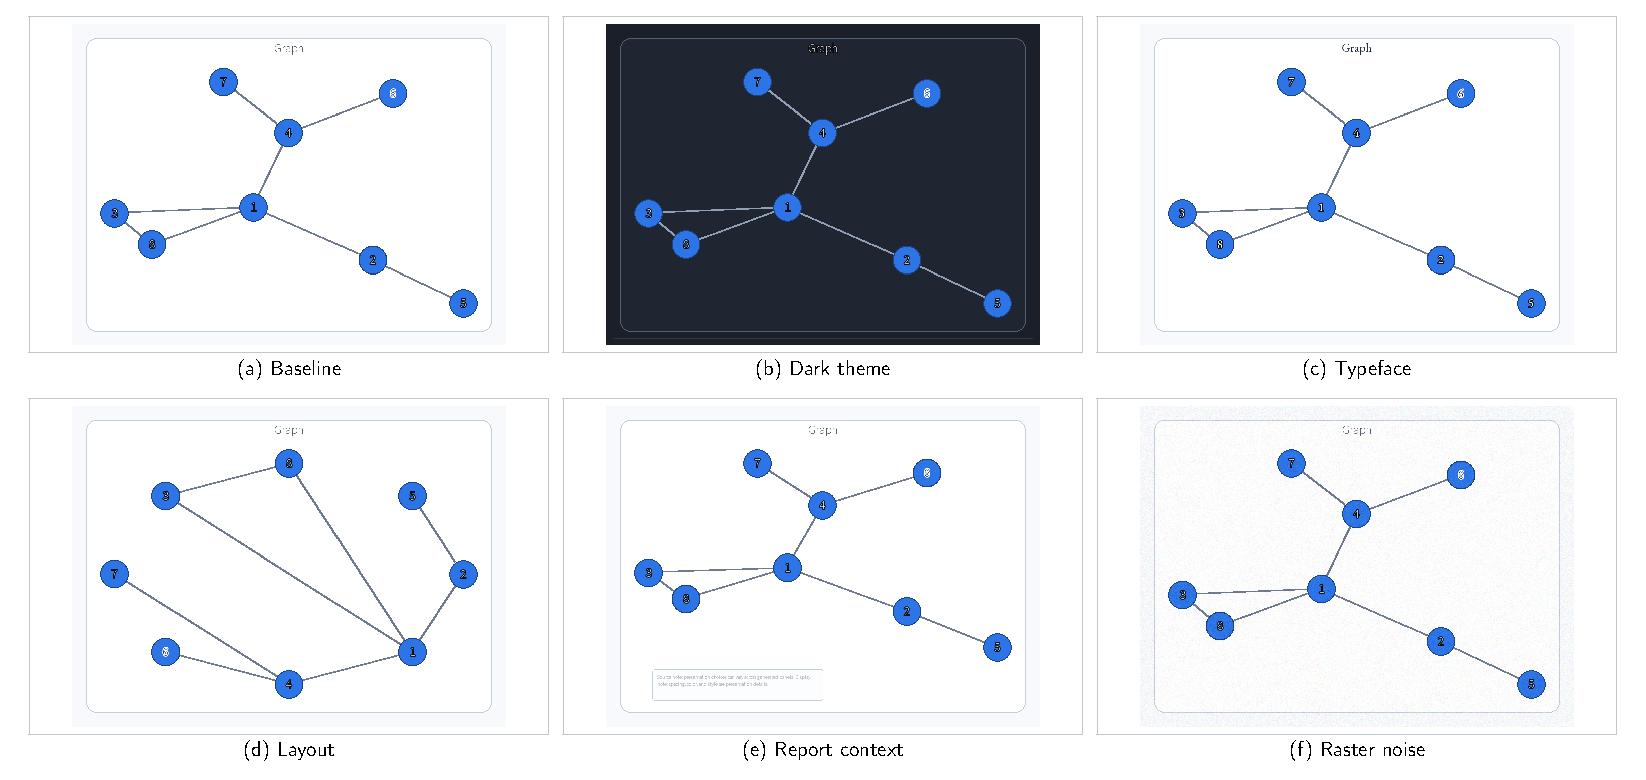
\includegraphics[width=\textwidth]{figures/rendering_variation_examples.pdf}
  \caption{One fixed semantic instance under controlled visual realization.
  Panels vary (a) the baseline style, (b) dark theme, (c) typeface, (d)
  graph layout, (e) non-answer report context, and (f) raster noise. Every
  panel retains the same task, query, prompt, graph topology, and typed
  answer; only the projected node positions and other controlled visual
  properties change.}
  \label{fig:rendering-variation}
\end{figure*}

\subsection{Validation and quality control}

Quality control combines construction-time constraints, contract validation,
deterministic replay, rendering checks, and human inspection. Before an
instance is retained, \trace verifies answer uniqueness, complete prompt
realization, reward compatibility, image and trace integrity, and agreement
between the answer and the recorded execution.

Automated checks establish structural invariants, but they cannot determine
whether a generated task is clear to a reader. Human inspection therefore
examines rendered samples for prompt clarity, visual legibility, answer
fitness, output distributions, taxonomy boundaries, and cross-sample
consistency. Separating these judgments from machine-checkable correctness is
important: a verifier can be internally consistent even when a visual problem
is ambiguous or unnecessarily difficult to read.

\FloatBarrier
